\documentclass[../TinyBot.tex]{subfiles}
\begin{document}

\section{Intro To Programming Arduinos}

To program an Arduino, you will need a USB cable, and a laptop/computer with the \href{https://www.arduino.cc/en/software}{Arduino IDE} installed. 



\begin{figure}[h]
    \centering
    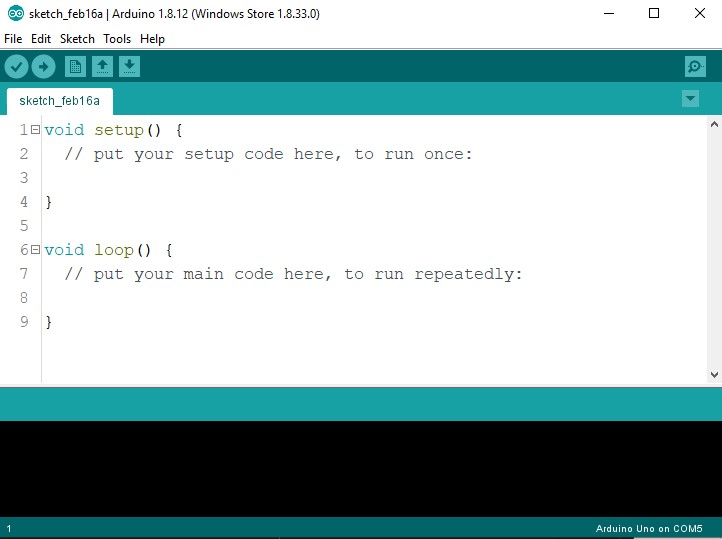
\includegraphics[width=0.7\textwidth]{arduino_ide.jpg}
    \caption{The Arduino IDE}
\end{figure}


Arduino's are programmed in the programming language \lstinline[]!C++!; though there are a few differences. The below code section details a few features of coding.


\begin{lstlisting}
// this is a comment

// variables declared not in a function will be accessible
// in all functions
int global_var = 0;

void setup {
  // everything in this function will run once
  // this code will run when the board is powered on, 
  // or when the reset button is pressed
}

void loop {
  // everything in this function will run repeatedly
}

\end{lstlisting}
\bigskip

\pagebreak
A useful feature of the Arduino IDE is all the example code which is provided.
\begin{figure}
    \centering
    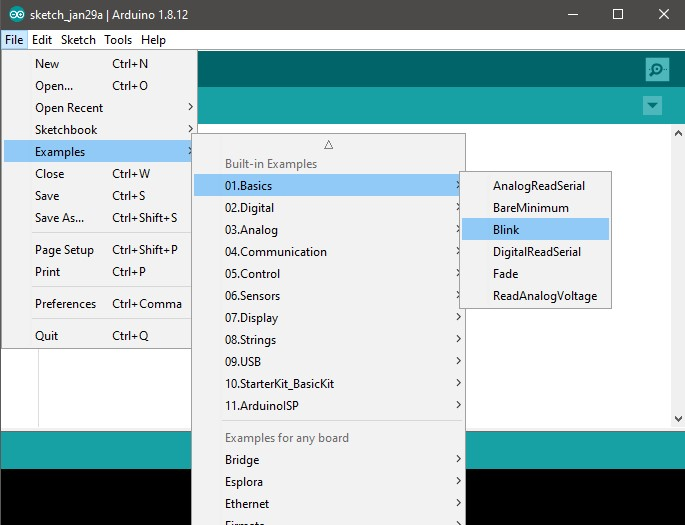
\includegraphics[width=0.8\textwidth]{arduino_ide_blink_example.jpg}
    \label{fig:ide-blink}
    \caption{Arduino IDE Example Code}
\end{figure}

The simplest Arduino example is the Blink code, which turns on and off an onboard LED.

\begin{lstlisting}
void setup() {
  // initialize digital pin LED_BUILTIN as an output.
  pinMode(LED_BUILTIN, OUTPUT);
}

// the loop function runs over and over again forever
void loop() {
  // turn the LED on (HIGH is the voltage level)
  digitalWrite(LED_BUILTIN, HIGH); 

  delay(1000);      // wait for a second

  // turn the LED off by making the voltage LOW
  digitalWrite(LED_BUILTIN, LOW);  
  
  delay(1000);      // wait for a second
}
\end{lstlisting}


There are a few common aspects present in the code of nearly every Arduino project, no matter how simple or complicated. \\


\lstinline[]!pinMode(<pin number>, <mode>)! sets a digital pin on the Arduino to be either an \lstinline[]!INPUT! or and \lstinline[]!OUTPUT!. \\


\lstinline[]!digitalWrite()! is used to set digital pins \lstinline[]!HIGH! and \lstinline[]!LOW!.

\end{document}